\documentclass[11pt, a4paper, twoside]{report}
\usepackage[utf8]{inputenc}
\usepackage[spanish]{babel}
\usepackage{lmodern}
\usepackage[T1]{fontenc}
\usepackage[top=2.5cm, bottom=2.25cm, outer=2.75cm, inner=2.75cm, heightrounded, marginparwidth=2.5cm, marginparsep=0.3cm]{geometry}	%márgenes
\usepackage{tabu}
\usepackage{pdfpages}
\usepackage{fancyhdr}

% Indicador completo en lugar de página
\fancyfoot[C]{{\ttfamily RTF PKT:CU \quad \thepage}}
\renewcommand*{\headrulewidth}{0pt}
\pagestyle{fancy}

\newcommand*{\PKT}{P\lower2pt\hbox{K}\kern-2pt\raise2pt\hbox{T}\kern-2pt}

\begin{document}

	% Título
	\begin{center}
		\scshape \large Acta de la Revisión Técnica Formal \textit{Casos de uso} - \PKT\ \vspace{.5cm}
	\end{center}

	En Madrid, a 8 de marzo de 2013 a la 13:02, reunidos de una parte Jaime Dan Porras, Alejandro Villarín Prieto e Ignacio Iker Prado Rujas representantes de \PKT\ y de otra Rubén Rafael Rubio Cuéllar y Juan Andrés Claramunt Pérez en representación de \textsc{Grupo Diedral}, se procede a la puesta en común de la revisión técnica formal de \textsc{Documento de casos de uso} de \PKT\ que \textsc{Grupo Diedral} ha realizado. \\

	Se presenta a la reunión por parte de \textsc{Grupo Diedral} el documento objeto de revisión con los apartados a comentar durante la reunión (se adjunta a este acta). \\


\noindent
A continuación se presentan los temas tratados y las conclusiones a las que se ha llegado,

	\begin{quotation} \itshape
			\textsc{Grupo Diedral} expone, \PKT\  toma notas y defiende su documento.

			\medskip
			Problemas generales

			\begin{enumerate}
				\item  La especificación de los casos de uso no se ajusta al esquema de los apuntes. En particular se hecha en falta el epígrafe de precondiciones que quedan incluidas, cuando quedan, de forma extraña en el propio ``curso típico de eventos''.
			Resolución: Se revisarán todos los casos de uso para que se ajusten a este esquema.
				\item Casi todos los casos de uso comienzan con el usuario registrándose en el sistema y acaban cerrando la aplicación. Esto parece demasiado drástico.
			Resolución: Paiky team está de acuerdo y lo cambiará en todos sus casos de uso.
				\item  La secuencia de acciones de muchos casos de uso relata el recorrido que ha hecho el usuario hasta llegar a la función, lo cual es irrelevante desde el punto de vista del caso de uso.
			Resolución: Se tratará de nuevo en todos los casos de uso.
				\item Se utilizan muchos términos tecnológicos como ``pestaña'', ``clica'', ``tacha'', ``tick'' ``pulsar'', ``botón'', ``cuadro de texto'', ``pinchar'' o ``ventana'' a lo largo de todo el documento.
			Resolución: Estos términos serán eliminados del documento.
				\item En general no queda claro por qué algunas secuencias son alternativas y no típicas.
			Resolución: Se aclararán los motivos por los que una secuencia es alternativa en un caso de uso.
				\item Faltan algunas tildes.
			Resolución: Gracias a que están marcadas por  \textsc{Grupo Diedral} en el documento escrito, se irán corrigiendo una a una.
				\item Errores concretos por inconsistencias que se detallan en el anexo.
			Resolución: Se corregirán en la siguiente revisión.
			\end{enumerate}

			\medskip
			Problemas concretos
			\begin{enumerate}
				\item Que el ``extracto'' sea una ``parte'' del documento puede resultar excesivo. Se puede hacer un \verb|\chapter*{Extracto}| o usar el entorno \verb|abstract|.
			Resolución: Se tendrá en cuenta cuando se revise la organización del documento.
				\item En el caso de uso 1.1. se dice ``Actores: Todos'' pero los actores no han sido presentado previamente.
			Resolución: Se presentarán previamente.
				\item En el caso 1.2. los campos no quedan muy claros, especialmente el de historial. En los cursos alternativos aparece que si no encuentra el nombre pregunta por el NIF; es decir, que si quieres buscar por el NIF tienes que escribir un nombre 				falso (anteriormente se usa DNI en lugar de NIF).
			Resolución: Paiky team acuerda cambiarlo.
				\item Caso 1.3: cuando el actor se equivoca al rellenar un campo, ¿el programa le informa de la causa del error?. Caso 2.5: ``los campos que sean necesarios'' no es preciso.
			Resolución: Paiky team considera que no tiene excesiva importancia.
				\item Casos 1.7, 1.14, 1.27, 2.11: están incompletos.
			Resolución: Ante la insistencia de  \textsc{Grupo Diedral}, se completarán los casos de uso indicados, o se moverán a secundarios.
				\item Caso 1.11: ejemplo de explicación de cómo se ha llegado hasta allí no conveniente. La interacción queda fijada como de tipo pregunta-respuesta por la redacción del curso típico.
			Resolución: Se corregirá en una posterior revisión.
				\item Caso 1.12: el título ``anular reserva'' no aclara, sin mirar al resto del documento, si se trata de una reserva de hotel de restaurante o ambas (igual con los siguientes). ¿Qué pasa si no hay reservas?
			Resolución: Paiky team acuerda solucionar la ambigüedad de alguna forma.
				\item Caso 1.13: se afirma que ``el programa manda el pedido a la cocina'', ¿cómo?. En el epígrafe 5 no queda muy claro qué es la carta y cómo se añaden o eliminan ingredientes.En los casos de contabilidad falta detalle.
			Caso 1.24: se refieren las ``características de las habitaciones'', ¿cuáles son?. Caso 1.25: está escrito ``se guarda toda la información de la reserva'', ¿qué información? Igualmente ``los campos a completar''.
			Caso 2.4: ¿de qué datos se compone un currículum?.
			Resolución: Paiky team choca frontalmente con los representantes de \textsc{Grupo Diedral}, pues opina que no son importantes esos detalles. Se determina que el Sr. Gonzalo resuelva el problema y se pasa al siguiente punto.
				\item Caso 1.15: se dice ``siempre que no haya empezado a prepararse'', ¿el programa sabe cuándo un plato está preparándose?
			Resolución: Se acuerda que Paiky team solucionará de alguna forma el problema, o eliminará el caso de uso.
				\item Caso 1.18 y 1.19: los nombres de los diagramas no coinciden con los nombres de los casos de uso en el texto del documento.
			Resolución: Se pide a  \textsc{Grupo Diedral} que no le comente nada a Gonzalo, y se compromete a modificar los diagramas.
				\item Caso 1.26: se llama ``ver reservas'' que no aclara por sí mismo si se trata de reserva de hotel o de restaurante. Además falta el correspondiente a reservas de restaurante. ``Se muestran la lista de reservas''.
			Resolución: Ambos son el  mismo, pues van juntas. En un futuro se tendrá en cuenta la opinión de Juanan para diferenciar unas reservas de otras.
				\item Caso 2.6: la ``visión general'' y el curso ``típico de los eventos'' son casi lo mismo.
			Resolución: Se cambiará la visión general para que no sea tan detallada.
				\item Caso 2.9: que una cantidad de algún elemento de las existencias no varíe, ¿no es típico? El ``introducir Intro'' induce a pensar que se tiene una interfaz de consola (desde luego es una referencia tecnológica indeseada).
			En cambio, marcar la opción ``Guardar y salir'' sugiere una interfaz gráfica.
			Resolución: Estos detalles de tan bajo nivel serán sustituídos por una descripción mediante un lenguaje más elevado.
				\item Caso 2.10 (añadir plato): la interacción es controlada rígidamente por el programa. ¿Qué son los ingredientes? ¿Están prefijados? Esa duda se resuelve en los cursos alternativos pero se introduce una base de datos: ¿es modificable? 					¿existe un caso de uso para ello?.
			Resolución: Se corregirá el caso de uso para que puedan introducirse manualmente los ingredientes y no tengan por qué estar prefijados. Añadiremos casos de uso secundarios que permitan editar la base de datos de ingredientes.
				\item Caso 2.10 (borrar plato): se afirma que el plato borrado queda almacenado en una base de datos para su posible uso posterior, pero no se explica cómo se recupera.
			Resolución: Un plato que se borre se eliminará sin quedar guardado.
				\item Caso 2.10 Deberían ser más de un caso de uso.
			Resolución: Se acuerda separarlos y añadir los que sean necesarios.
				\item Parte de lo dicho de algunos casos particulares se puede aplicar en otros.
			Resolución: Se le dará una pasada al documento corregido y se modificarán los casos de uso en los que esté indicado algún error de los que se han aceptado corregir en los puntos anteriores.
			\end{enumerate}

	\end{quotation}

	\noindent
	Por tanto, el documento se declara \textsc{rechazado}.\\
	Ambas partes expresan la conformidad con lo hablado en la reunión.

\vspace{2cm}
\raggedleft{En Madrid, a 8 de marzo de 2013}

\raggedright
Los asistentes,

\vspace{2.5cm}

	\begin{tabu} to \linewidth {X[1,c] X[1, c] X[1, c]}
		Jaime Dan Porras & Alejandro Villarín Prieto & Iker Ignacio Prado Rujas
	\end{tabu}

	\vfill

	\begin{tabu} to \linewidth {X[1,c] X[1, c]}
		Rubén Rafael Rubio Cuéllar & Juan Andrés Claramunt Peréz
	\end{tabu}
	
	\vfill

	{\itshape A continuación se incluye el anexo elaborado por el equipo revisor: }

	% Incluye el anexo del otro grupo
	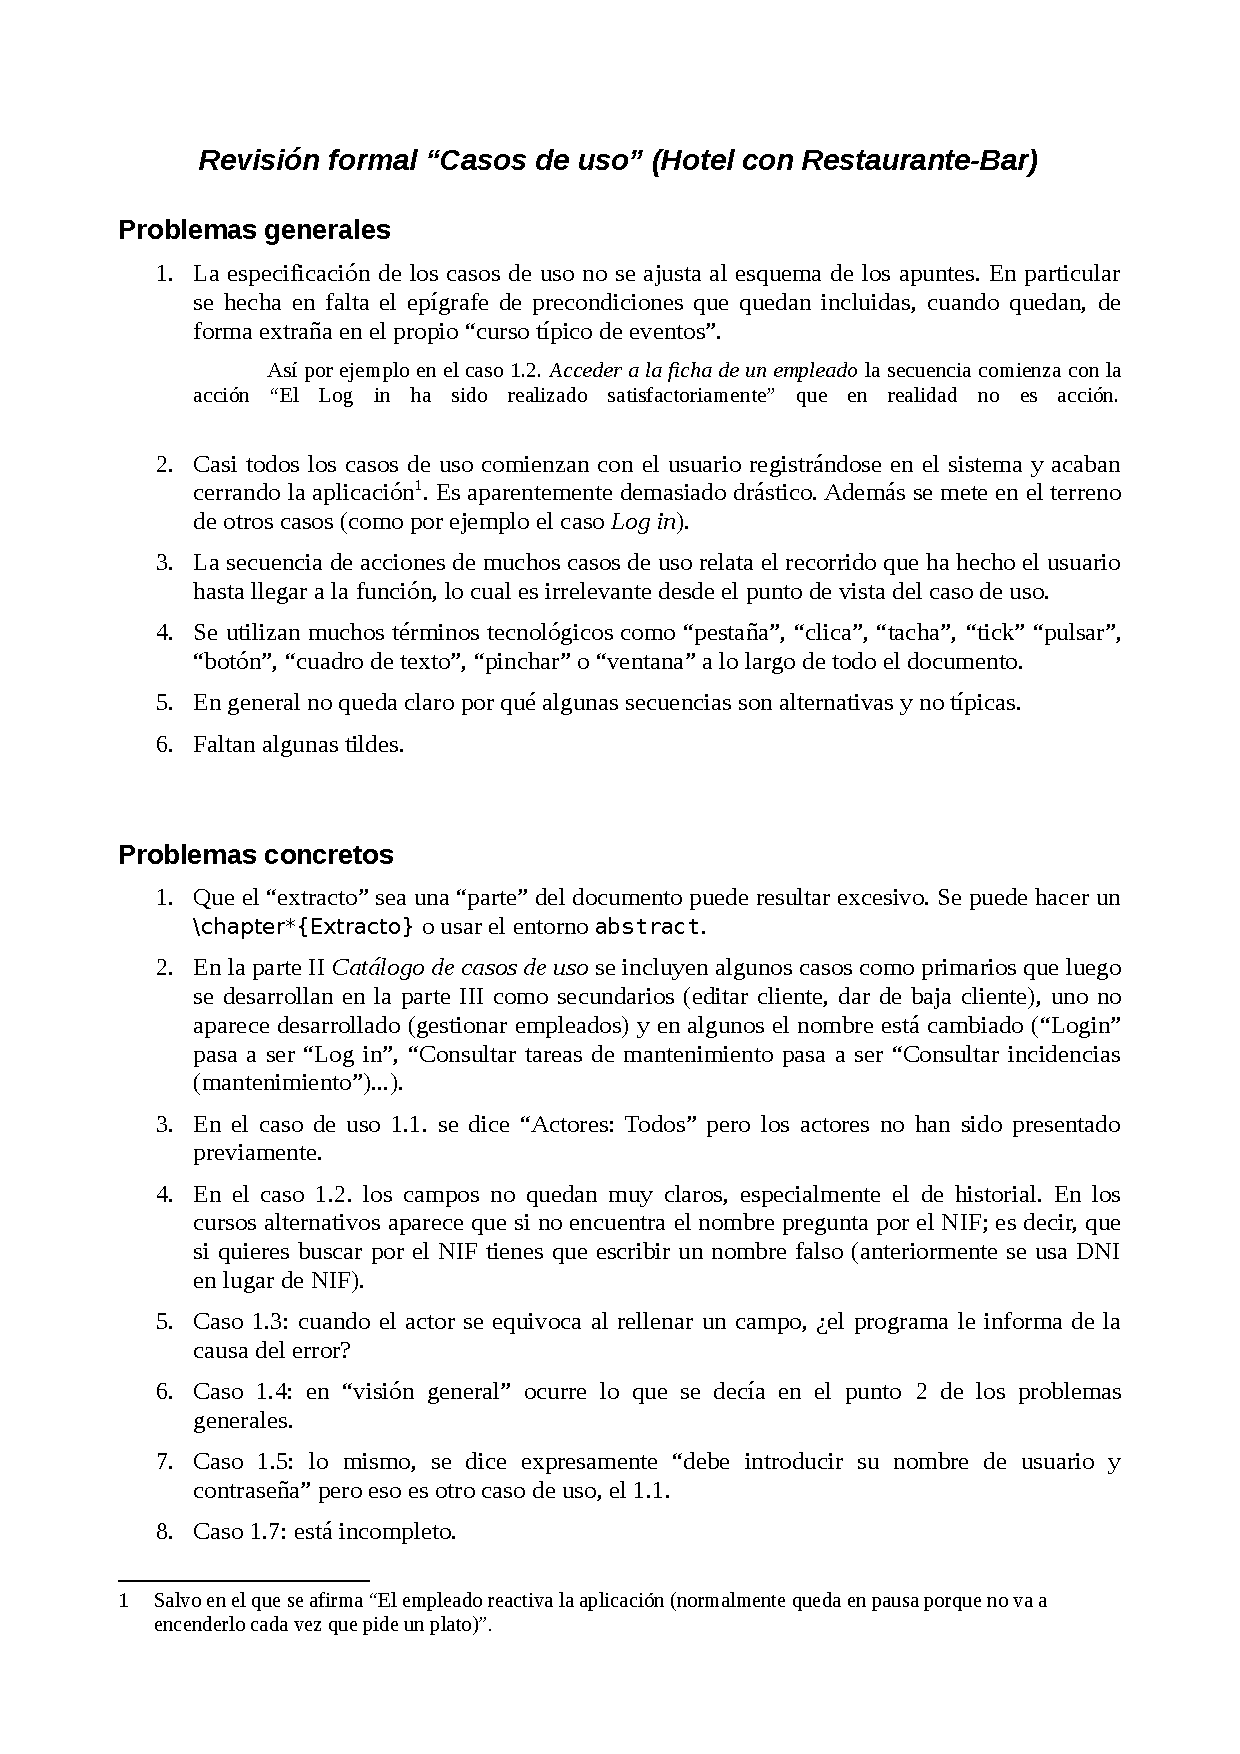
\includepdf[pages=1-2, pagecommand={}]{casosdeuso_pkt_anexo.pdf}
\end{document}
